%!TEX root = ../../thesis.tex
%*******************************************************************************
%****************************** Solution Implementation Chapter *********************************
%*******************************************************************************

\chapter{Solution Implementation}

\ifpdf
    \graphicspath{{Chapters/Implementation/Figs/}{Chapters/Implementation/Figs/}{Chapters/Implementation/Figs/}}
\else
    \graphicspath{{Chapters/Implementation/Figs/}{Chapters/Implementation/Figs/}}
\fi
In the previous chapter, we displayed an overview design of our approach.
Consequently, the solution implementation chapter of this thesis presents the details of how the proposed system was developed and implemented.
Firstly, we define some \ac{df} (see section \ref{implementation:section:designfeatures}) that focus on designing and developing new artifacts, methods, or systems.
It begins with a description of the system's architecture (see section \ref{implementation:section:architecture}), including the major components and their interactions.
Next, the description of the technology stack and development tools is explained (see section \ref{implementation:section:technologies}).
The chapter includes a detailed explanation of the critical features and functionality of the system and the processes used in frontend implementation (see section \ref{implementation:section:frontend}), database implementation (see section \ref{implementation:section:database}) backend implementation (see section \ref{implementation:section:backend}), and the software tool (see section \ref{implementation:section:tool}).
Through this chapter, readers will understand how we brought the proposed solution to reality and its potential for real-world applications.

\section{Platform Design Features (DFs)}
\label{implementation:section:designfeatures}
\ac{dsr} aims to produce a tangible outcome, such as a new software tool, a process improvement, or a theoretical framework.
It often involves multiple cycles of design, evaluation, and redesign, allowing for constant improvement of the artifact.
Since we perform the \textit{first} iteration of the cycle, we derive the features of our software tool using the \ac{df}s.
In this section, we translate each \ac{dp}s (we defined in chapter \ref{chap:design}) into a set of \ac{df}s that we can directly implement into the tool or solution approach and we describe the \ac{df}s for each of the derived \ac{dp}s.
As shown in the figure \ref{fig:implementation:hierarchy}, we see that the \ac{df}s are divided according to the \textit{LEAN} development cycle.
\clearpage
\begin{landscape} 
\begin{figure}[htbp!]
    \centering
    \begin{subfigure}[b]{1.0\textwidth}
    \centering
    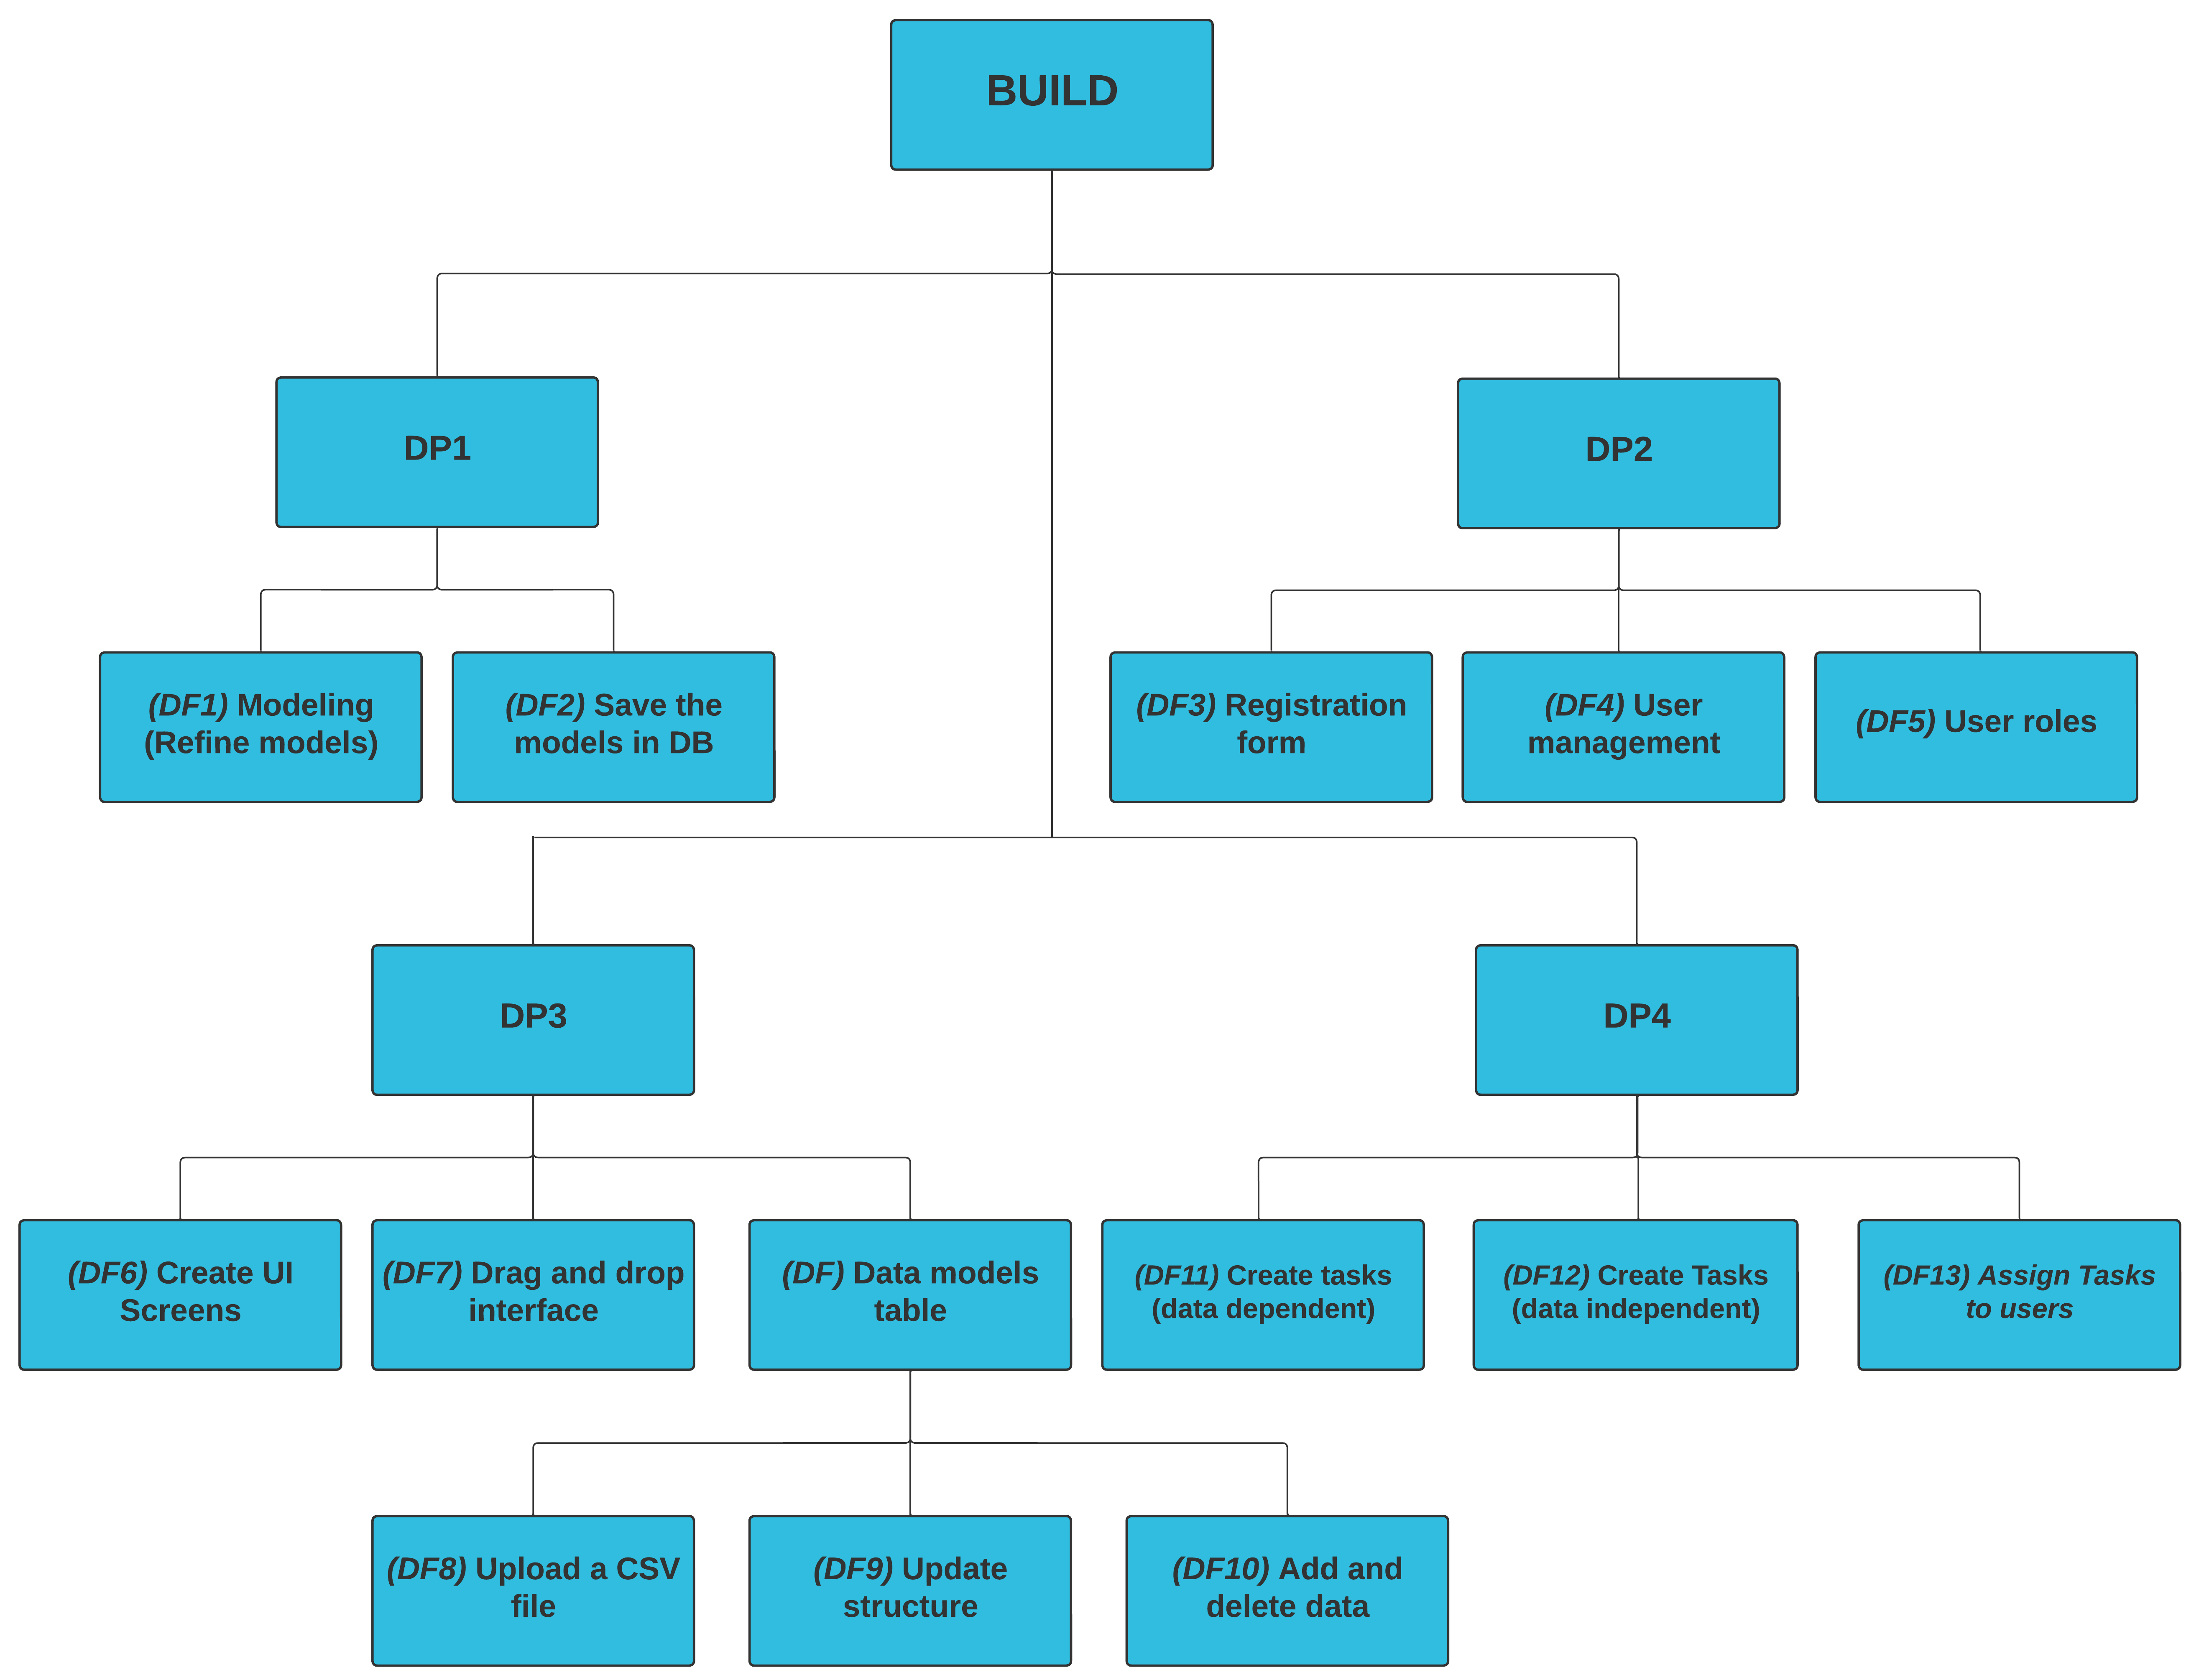
\includegraphics[width=1.2\textwidth]{DFs_hierarchy_build.png}
    \caption{A hierarchical diagram of \ac{df}s from \textit{Build} phase}
    \label{fig:implementation:hierarchy:build}
    \end{subfigure}
    \begin{subfigure}[b]{1.0\textwidth}
    \centering
    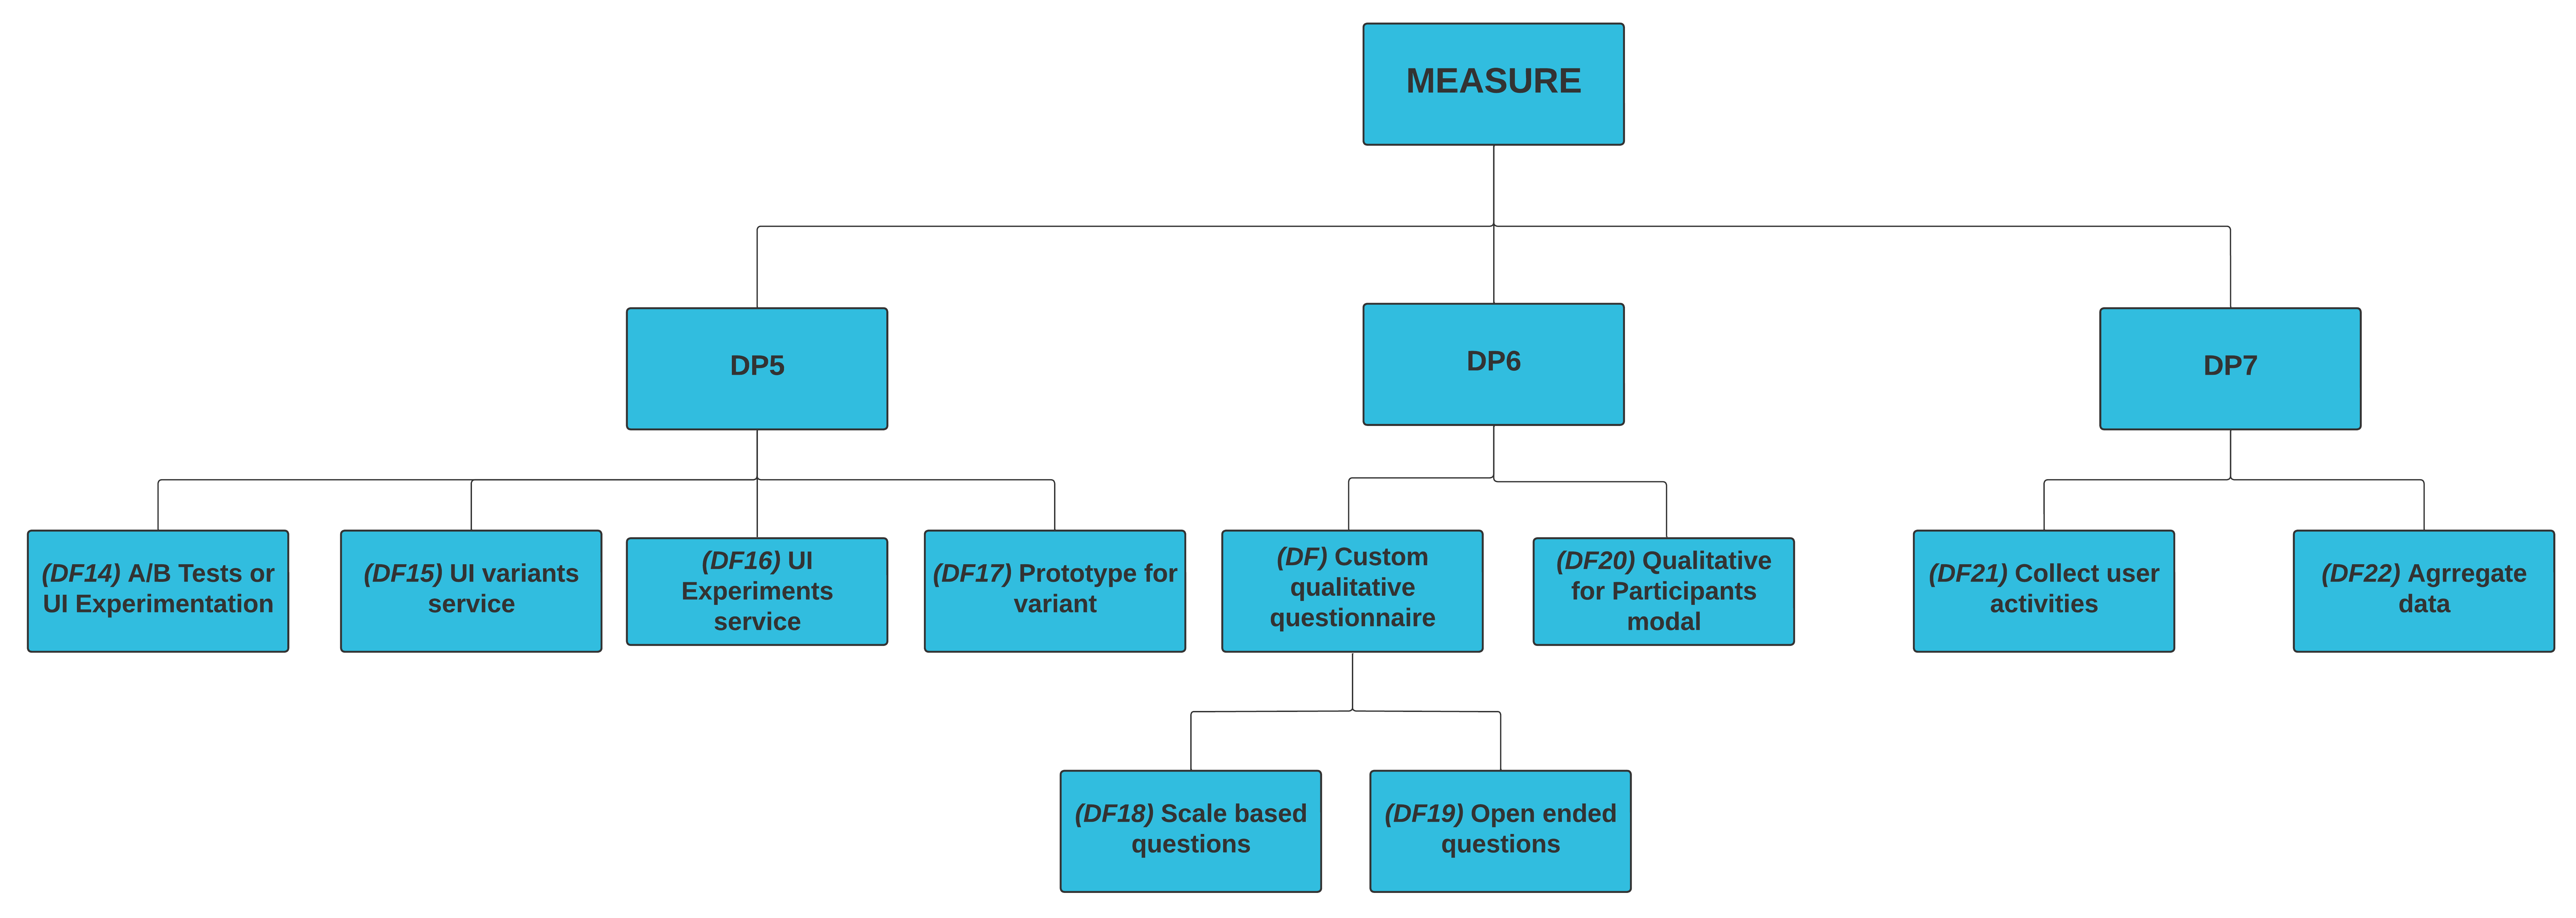
\includegraphics[width=0.8\textwidth]{DFs_hierarchy_measure.png}
    \caption{A hierarchical diagram of \ac{df}s from \textit{Measure} phase}
    \label{fig:implementation:hierarchy:measure} 
    \end{subfigure}             
    \begin{subfigure}[b]{0.8\textwidth}
    \centering
    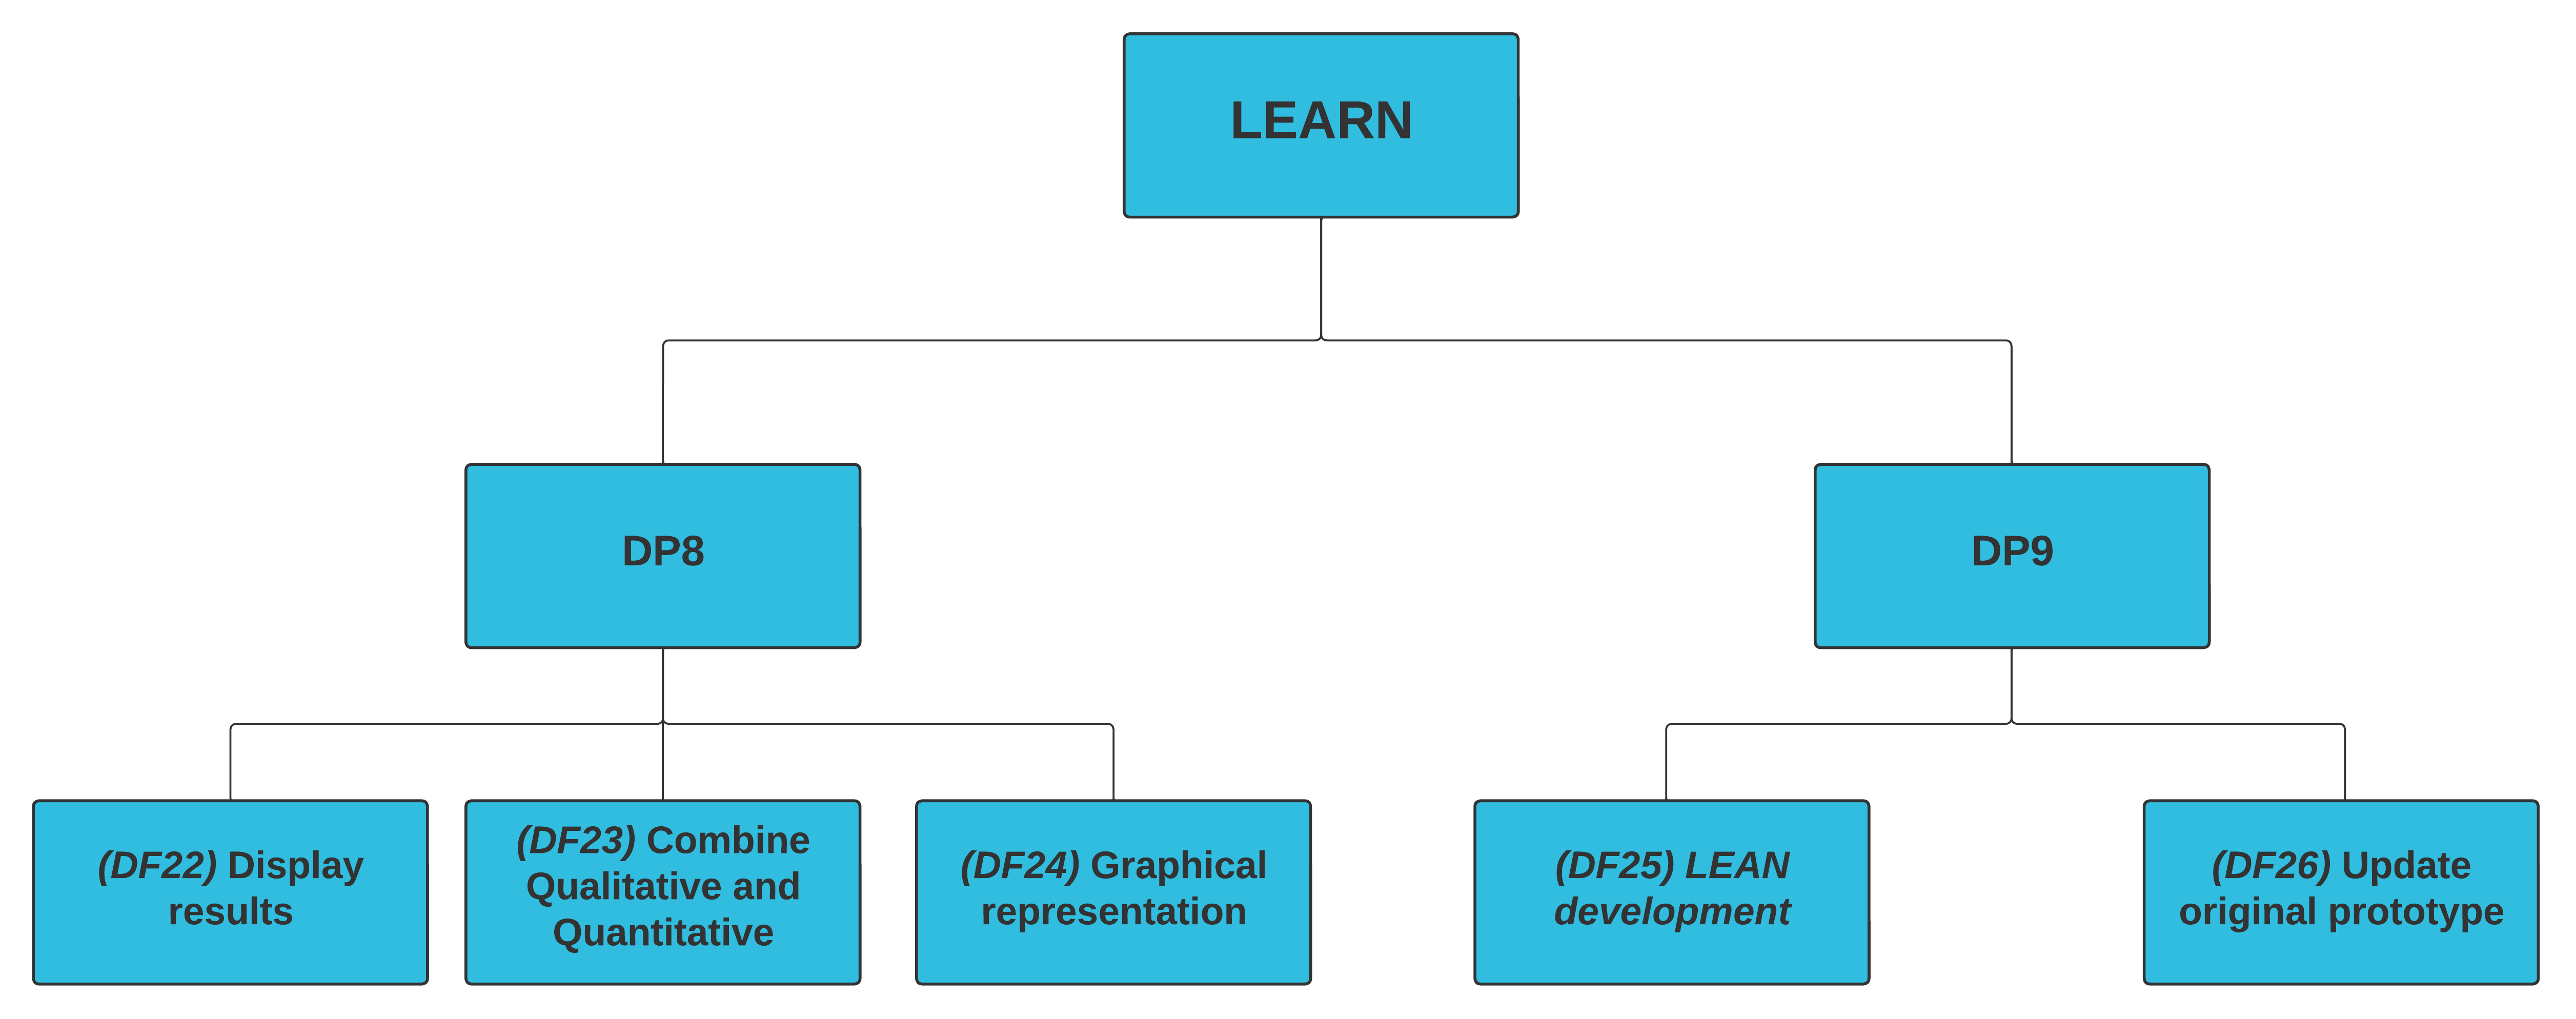
\includegraphics[width=0.7\textwidth]{DFs_hierarchy_learn.png}
    \caption{A hierarchical diagram of \ac{df}s from \textit{Learn} phase}
    \label{fig:implementation:hierarchy:learn}
    \end{subfigure}
    \caption[A map between \ac{dp}s and \ac{df}s]{Hierarchical structure of \ac{df}s}
    \label{fig:implementation:hierarchy}
\end{figure}
\end{landscape}
\paragraph{Build:}
In the \textit{Build} phase of the \textit{LEAN} development cycle, based on the \textbf{\ac{dp}1: Modeling}, the solution approach provides features for creating the models (\textit{\ac{df}1}) useful for persisting data in the database and updating them (\textit{\ac{df}2}) with the results of the experiments.
It helps to create our prototypes in a model-based approach and improve our prototypes by improving the models throughout the LEAN development cycle.
With the \textbf{\ac{dp}2: User Variety}, the key features of our solution approach for the \ac{ui} prototyping tool will include registration for diverse users using a registration form (\textit{\ac{df}3}) and user management, i.e., features that enable team members to create and manage user accounts (\textit{\ac{df}4}), assign different levels of access and permissions (\textit{\ac{df}5}).
The \textit{User module} maintains all these features and also the user authentication, authorization, and user profile management.
And then based on the \textbf{\ac{dp}3: Flexible UI Elements}, the privileged user prototypes using the features of our solution approach, which includes the creation of different screens (\textit{\ac{df}6}) and reusable \ac{ui} elements using a drag and drop interface (\textit{\ac{df}7}). 
The tool also provides a feature to add custom data i.e., creating data models by uploading a \ac{csv} file (\textit{\ac{df}8}), revising structures of data model table (\textit{\ac{df}9}), adding and deleting data from the table (\textit{\ac{df}10}).
Next, based on the \textbf{\ac{dp}4: User tasks Refinement}, the privileged user creates \textit{User Tasks} for the users using the features of our solution approach, which includes creating tasks for users depending on the data model (\textit{\ac{df}11}) and independent of data models (\textit{\ac{df}12}), and assign the task to the experiments (\textit{\ac{df}13}).

\paragraph{Measure:}
In the \textit{Measure} phase of the \textit{LEAN} development cycle, based on the \textbf{\ac{dp}5: Split Tests}, the privileged user would be able to create A/B tests or \ac{ui} experimentation (\textit{\ac{df}14}) using the features of our solution approach, which includes creating and modifying the experiments (\textit{\ac{df}15}), creating and updating the \ac{ui} variants (\textit{\ac{df}16}), and modifying the variants' prototypes such that each variant has a unique view (\textit{\ac{df}17}).
Next, based on the \textbf{\ac{dp}6: Qualitative Analysis}, the privileged user would be able to do qualitative analysis on the users using the features of our solution approach, which includes creating the custom qualitative questionnaire with options in the answering formats like \textit{Scale based}, i.e., the users will have to choose from options 1 to 10 (\textit{\ac{df}18}) and open-ended questions, i.e., the users will have the freedom to answer whatever they think (\textit{\ac{df}19}). 
And, the users will answer these questions after finishing the tasks with a modal appearing with different questions (\textit{\ac{df}20}). 
Similarly, based on the \textbf{\ac{dp}7: Quantitative Analysis}, the privileged user creates quantitative analysis on the users using the features of our solution approach, which includes collecting the task data feedback, i.e., collecting the time taken to finish the task, number of unsuccessful attempts, the path taken by the users to complete the task, etc. (\textit{\ac{df}21}), and aggregating these feedback data (\textit{\ac{df}22}). 

\paragraph{Learn:}
In the \textit{Learn} phase of the \textit{LEAN} development cycle, based on the \textbf{\ac{dp}8: Diversity in Analysis}, the privileged user compares the statistics using the features of our solution approach, which includes showing the results of the experiment (\textit{\ac{df}23}), combining qualitative and quantitative analysis of each variant (\textit{\ac{df}24}), and a graphical view to see the results (\textit{\ac{df}25}). 
Finally, based on the \textbf{\ac{dp}9: Continuous Design}, the solution approach would provide features including LEAN development cycle (\textit{\ac{df}26}). 
The privileged user should be able to update the original prototype with the results from the experiment (\textit{\ac{df}27}) for continuous improvement.

Overall, the design features section in DSR delivers a comprehensive overview of the solution tool to address the identified problem or research question. 
Moreover, this section describes the \ac{df}s for our \ac{poc} solution tool.
\clearpage

\section{Technologies Used}
\label{implementation:section:technologies}
We have created a software tool that allows us to test the features (\ac{df}s) and underlying principles of the developed DFs with actual users.
To test our solution approach, we developed a rapid prototyping tool for the first cycle of our \ac{dsr}. 

The implementation of our \textit{UI Prototyping Tool with Experimentation (UPTE)} platform uses various technologies.
Our UI prototyping tool was developed using Angular\footnote{A framework of javascript: \url{https://angular.io/}}, Loopback\footnote{A framework of the NodeJS \url{https://loopback.io/}}, and MongoDB\footnote{A non-relational database \url{https://www.mongodb.com/}}.
Angular is a JavaScript framework used for building web-based applications.
It provides comprehensive tools for creating dynamic and responsive UI components and handling user interactions.
With angular, we are using several other UI components which are available on Node package manager (npm)\footnote{NPM: \url{https://www.npmjs.com/}}.

Loopback is a Node.js\footnote{NodeJS: \url{https://nodejs.org/en/}} framework used for building RESTful APIs. 
It provides an intuitive interface for creating API endpoints and managing data persistence. 
Loopback's support for various data sources, including relational and NoSQL databases, makes it a versatile choice for web applications. 
We connect our database using the data managers provided by the loopback framework.
The framework's ability to generate API documentation and testing tools simplifies our development process.

MongoDB is a NoSQL document-oriented database used for storing unstructured data. 
We store our prototyping tool's data using a JSON\footnote{What is JSON: \url{https://developer.mozilla.org/en-US/docs/Glossary/JSON}} format in an unstructured manner.
It provides a scalable and flexible solution for managing volumes of data. 
MongoDB's support for automatic sharding and replication ensures high availability and fault tolerance. 
The database's dynamic schema and rich query language make it easy to adapt to changing data requirements.

By leveraging these technologies, our UI prototyping tool delivered a powerful and user-friendly interface while ensuring efficient data retrieval and storage.
Based on these technologies, we build a microservice architecture explained in the next section so that our \ac{dp}s and \ac{df}s can be easily implemented. 
\clearpage

% \section{Solution Architecture}
% \label{implementation:section:architecture}

\section{Frontend Implementation}
\label{implementation:section:frontend}

\section{Database Schema}
\label{implementation:section:database}

\section{Backend Implementation}
\label{implementation:section:backend}

\section{Software Tool}
\label{implementation:section:tool}